\section{Wellenleiter}
\subsection{Koaxial Leiter}
\subsubsection{Wellenwiderstand}

\begin{center}
    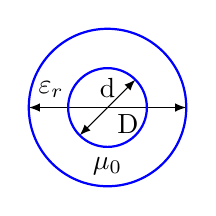
\begin{tikzpicture}
        \draw[latex-latex](-1,0)node[above right]{$\varepsilon_r$}--(1,0);
        \node[below right, yshift=1pt]{D};
        \draw[latex-latex, rotate=45](-0.5,0)--(.5,0);
        \node at (0,0)[above]{d};
        \draw[-, thick, blue](0,0) circle (1);
        \node at(0,-.75)[]{$\mu_0$};
        \draw[-, thick, blue](0,0) circle (0.5) ;
    \end{tikzpicture}


    D = Außendurchmesser

    d = Innendurchmesser
\end{center}
\vspace{-1em}

\begin{align*}
    Z_L = \frac{60\Omega}{\sqrt{\varepsilon_r}}\cdot \ln{\frac{D}{d}}
\end{align*}

\subsubsection{Dämpfung}
\underline{\textbf{Ohm'sche Verluste}} $R\ll\omega L$
\begin{align*}
    \alpha_0 = \frac{\sqrt{\frac{f\cdot\mu}{\pi\cdot\sigma}}}{120\Omega}\cdot\frac{\sqrt{\varepsilon_r}}{D}\cdot\frac{1+\frac{D}{d}}{\ln \frac{D}{d}}
\end{align*}

\underline{\textbf{Dielektrische Verluste}} $G\ll\omega C$,$\tan\delta= (^G/_{\omega C})$
\begin{align*}
    \alpha_d = \pi\sqrt{\varepsilon_r}\cdot\tan\delta\cdot\frac{f}{c_0}
\end{align*}

\subsection{Mikrostreifenleiter}
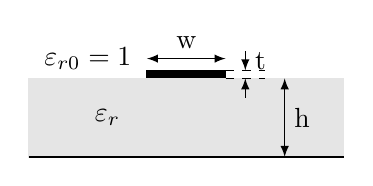
\begin{tikzpicture}
    %Leiterbahn
    \filldraw[black]    (1,1)   rectangle (2,1.1);
    %Dielektrika
    \filldraw[black!10] (-.5,0) rectangle (3.5,1);
    \draw[-,thick](-.5,0)--(3.5,0);
    %Bemassungen
    \draw[latex-latex](2.75,0)--(2.75,1) node[midway, right]{h};
    \draw[latex-latex](1,1.25)--(2,1.25) node[midway, above]{w};
    \draw[dashed](2,1)      --(2.5,1);
    \draw[dashed](2,1.1)    --(2.5,1.1);
    \draw[latex-](2.25,1)   --(2.25,.75);
    \draw[latex-](2.25,1.1) --(2.25,1.35) node[midway, right]{t};
    %Dielektrizitätskonstanten
    \node at (.5,.5)[]{$\varepsilon_r$};
    \node at (.25,1.25)[]{$\varepsilon_{r0}=1$};
\end{tikzpicture}

\subsubsection{Effektive Permittivitätszahl}
\begin{align*}
     & \text{Unterschiedliche Phasengeschwindigkeit $\rightarrow$ Dispersion}                                              \\
     & \varepsilon_{r,eff}  = \frac{\varepsilon_r+1}{2}+\frac{\varepsilon_r-1}{2\sqrt{1+10\cdot\frac{\text{h}}{\text{w}}}} \\
     & \text{Je größer $\frac{\text{w}}{\text{h}}$ desto mehr nähert sich $\varepsilon_{r,eff}$ an $\varepsilon_r$ und}    \\
     & \lambda              = \frac{\lambda_0}{\sqrt{\varepsilon_{r,eff}\cdot\mu_{r,eff}}}
\end{align*}
\subsubsection{Schmale Streifen}
\begin{align*}
    Z_L & = \frac{60\Omega}{\sqrt{\varepsilon_{r,\texttt{eff}}}}\cdot\ln\left(\frac{8\text{h}}{\text{w}}+\frac{\mathrm{w}}{4\mathrm{h}}\right)
\end{align*}
\subsubsection{Breite Streifen}
\begin{align*}
    Z_L & = \frac{120\pi\Omega}{\sqrt{\varepsilon_{r,\texttt{eff}}}}\cdot\frac{1}{\frac{\text{w}}{\text{h}}+2,42-0,44\cdot\frac{\mathrm{h}}{\mathrm{w}}+\left(1-\frac{\mathrm{h}}{\mathrm{w}}\right)^6}
\end{align*}

\subsection{Hohlleiter}
\begin{align*}
    f_c & = \frac{c_0}{2a}
\end{align*}

\subsection{VSWR (Voltage Standing Wave Ratio) und Return Loss}
\begin{align*}
    s        & = VSWR = \frac{1+|r|}{1-|r|}\geq 1 \\
    |r|      & = \frac{s-1}s+{1}                  \\
    \alpha_r & = -20\log(r)dB                     \\
             & \text{Missmatch Loss}              \\
    ML       & = -10\log(1-r^2)dB
\end{align*}
